\section{Planar\-CDI.h File Reference}
\label{PlanarCDI_8h}\index{PlanarCDI.h@{PlanarCDI.h}}
{\tt \#include \char`\"{}Base\-CDI.h\char`\"{}}\par


This graph shows which files directly or indirectly include this file:\begin{figure}[H]
\begin{center}
\leavevmode
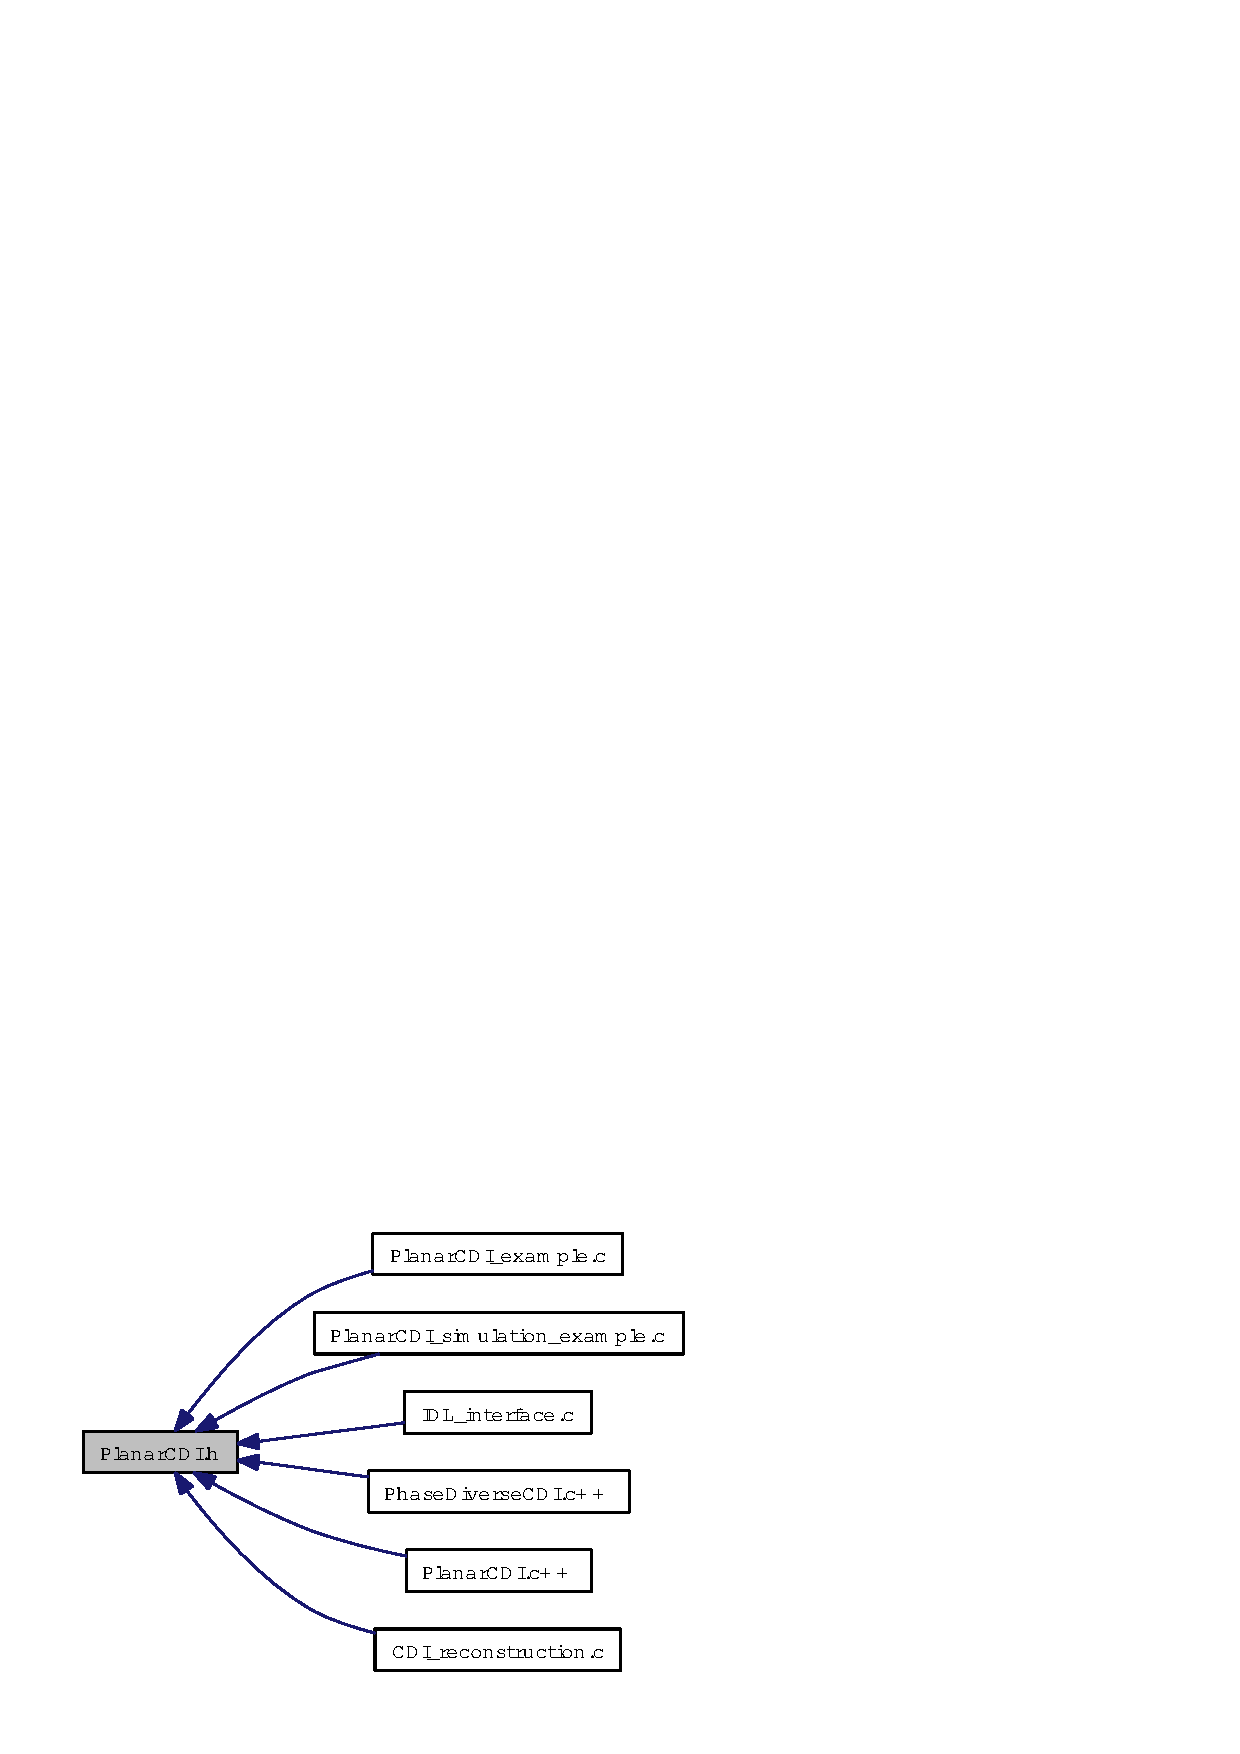
\includegraphics[width=166pt]{PlanarCDI_8h__dep__incl}
\end{center}
\end{figure}
\subsection*{Data Structures}
\begin{CompactItemize}
\item 
class \bf{Planar\-CDI}
\begin{CompactList}\small\item\em The class which performs planar CDI reconstruction. \item\end{CompactList}\end{CompactItemize}


\subsection{Detailed Description}


Definition in file \bf{Planar\-CDI.h}.